% !TEX root = ../Documentation.tex

\section{Test Report}
\label{sec:tests}

\subsection{Test suite}
  Together with the new parser, a test suite has been developed.
  This test suite has been used to verify the performance and correctness of the new parser.
  The source code can be found in the folder \texttt{src/Database/Design/Ampersand/Test} within the Ampersand repository.

  The test suite runs in three steps, which are depicted in \autoref{fig:TestModules}.
  Each of the modules are described in the following subsection.
  %
  \begin{figure}[ht]%
    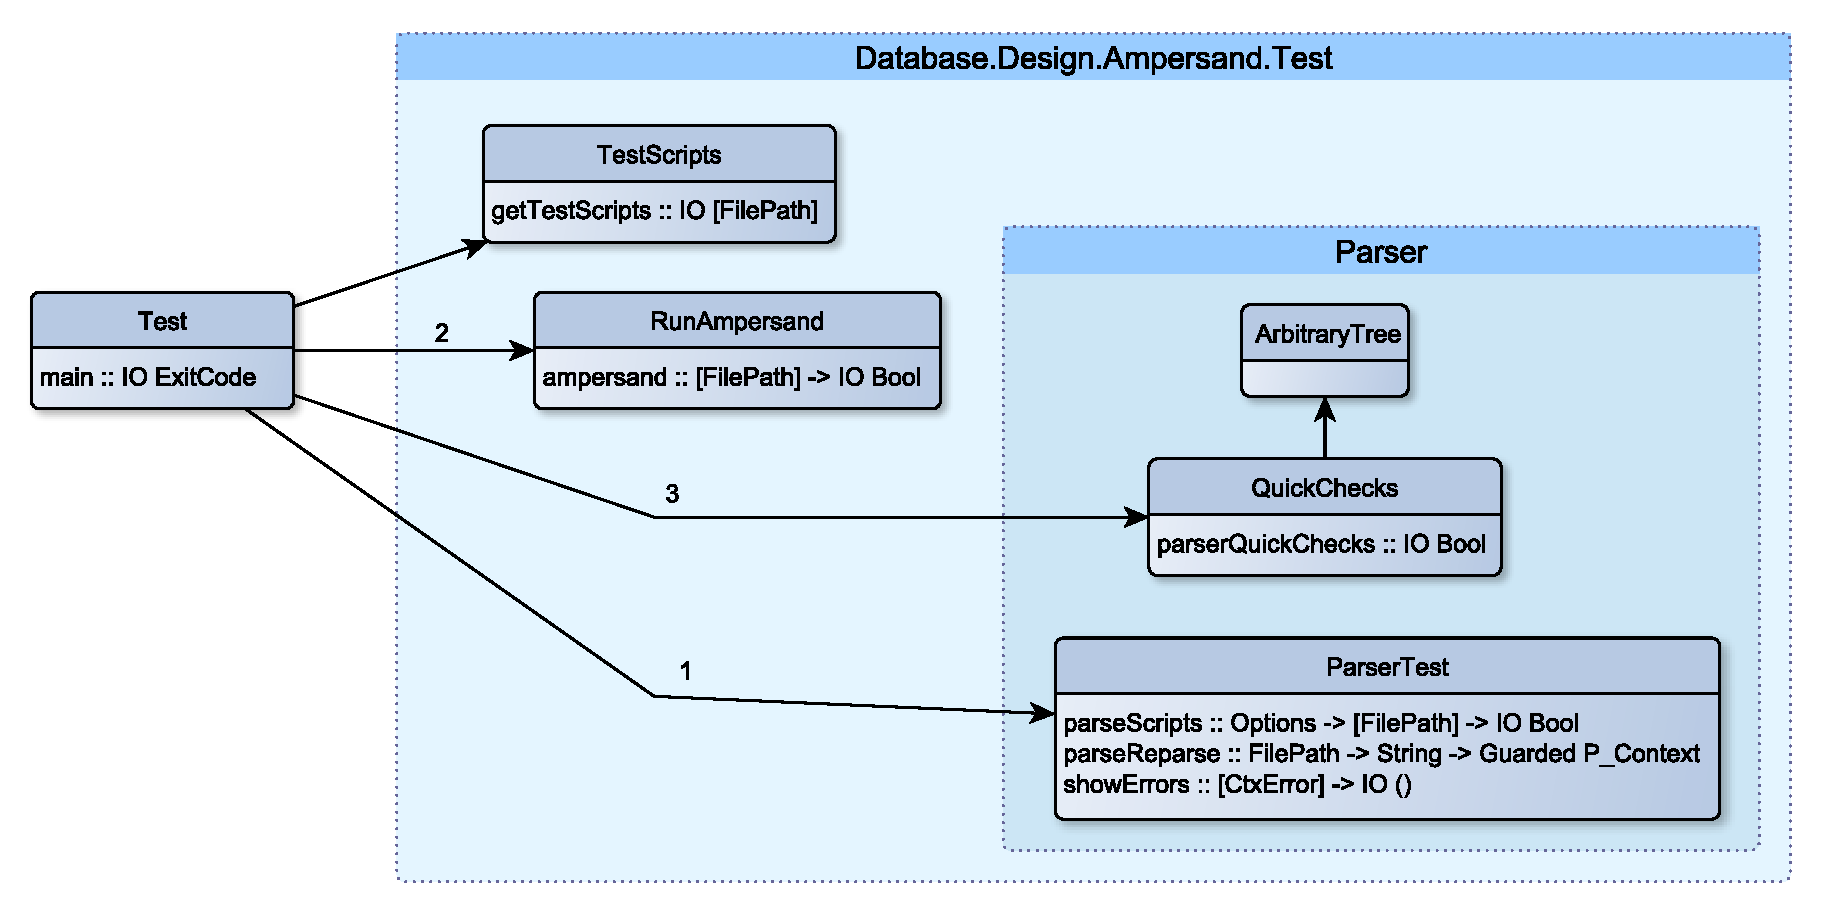
\includegraphics[width=\columnwidth]{Figures/TestModules}
    \caption{Test suite modules with their exported functions}
    \label{fig:TestModules}
  \end{figure}%

  \subsubsection{Modules}
  \label{subsec:test-modules}
  In this section a short description of each module is given:%
  %
  \begin{description}
    \item[Test] contains the \texttt{main} method that can be executed to run the test suite.
      The \texttt{main} function calls each of the other modules in sequence, stopping if any of them returns \texttt{False}.
      When all tests have been successful, the return code is \texttt{ExitSuccess}.
      Otherwise, the return code is naturally \texttt{ExitFailure}.
    
    \item[TestScripts] retrieves a list of scripts that can be used for the different tests.
      It searches for tests within the folder \texttt{ArchitectureAndDesign}, and contains a list of scripts from the \texttt{ampersand-models} repository, that can be changed at a later moment if wished.
      Note that all the ADL-scripts listed in this section must be correct for the parser and the type checker.
    
    \item[ParserTest] exports three functions that are the core of testing the parser:
      \begin{itemize}
        \item \texttt{parseScripts} receives a list of files to parse, and checks that every file can be parsed successfully.
        \item \texttt{parseReparse} tries to parse a file, and if sucessfull, pretty-prints the result and parses it again.
        \item \texttt{showErrors} prints the given parse errors to the output.
      \end{itemize}
    
    \item[RunAmpersand] receives a list of files, and checks that every file can be executed successfully by Ampersand.
      This tests thus not only the parser, but also the interface between the parser and the type checker, as the rest of the Ampersand chain.
    
    \item[QuickChecks] generates random parse tree structures and generates the corresponding ADL-script by pretty printing the parse tree.
      This ADL-script is then fed back to the parser through the \texttt{parseReparse} function, to verify that the parser can accept any random input.
      More information on the quick checks is given in subsection~\ref{subsec:quick-check}.
    
    \item[ArbitraryTree] is a support module that gives \texttt{Arbitrary} instances to all parse-tree structures.
      This is used by QuickCheck as described in subsection~\ref{subsec:quick-check}.
    
    \item[ArbitraryPandoc] contains \texttt{Arbitrary} instances to the Pandoc data types.
      This file has not been developed in this project, but copied from the \texttt{jgm/pandoc} project with the GPL license.
  \end{description}

  \subsubsection{QuickCheck and pretty printing}
  \label{subsec:quick-check}
  The most innovative part of the test suite is the use of random structures to test the parser.
  In this section we describe how this generation is implemented.
  
  The main role in the generation of random structures is played by the support library QuickCheck, which has been added to the Ampersand project.
  QuickCheck is able to generate any data structure randomly.
  However, since the parse tree is a custom structure that must obey specific rules, QuickCheck requires the specification of these rules by instances of the \texttt{Arbitrary} class.
  
  Every data structure in the parse tree has received an \texttt{Arbitrary} instance used for test purposes.
  The instances can be found in the module \texttt{Database.Design.Ampersand.Test.Parser\-.ArbitraryTree}, as described in subsection~\ref{subsec:test-modules}.
  
  After generating the random parse trees, the test suite needs to convert them to ADL-scripts.
  The conversion of parse tree to source code is also known as pretty printing.
  As the pretty printing is seen as part of the parse tree, it is not included in the Test modules, but is part of the input subsystem.
  The pretty printing instances are found in the module \texttt{Database.Design.Ampersand.ADL1.PrettyPrinters}.
  This module makes use of the library \texttt{Text.PrettyPrint.Leijen}, that outlines the output so it is indeed `pretty'.
  
  Now that the ADL source is available, the parser is executed.
  The result of the parser is checked to be equal to the generated tree by the property \texttt{prop\_pretty}.
  The property is currently tested for 64 generated parse trees in the test suite.
  If the test fails for any generated structure, the test suite fails with an appropriate error.
  
  \subsubsection{Running the tests}
  During the parser development, the \texttt{main} function of the parser tests has been executed manually, through a batch file.
  This is mainly done because the project team did not have access to the Sentinel server, and no documentation was available on how to run Sentinel locally in a Windows machine.
  However, now that the parser is being delivered, it should be integrated with the other existing Ampersand/Sentinel tests.
  We leave the option open for the Ampersand development team to either add the Sentinel jobs to this test suite, or to add the parser test suite to the Sentinel jobs.
  
\subsection{Errors}
  Since evaluating the quality of error messages is manual work, the errors have not been included in the test suite.
  TODO: Give Maarten's findings on how the errors have improved. Maybe the tables should be an attachment, but the summary should be here.

\subsection{Next steps}
  In this section we name a couple changes that can be done in the test suite in the future:
  \begin{description}
    \item[Sentinel] During the development of the new parser, we worked in a separate fork.
      Our changes were not being tested in the Ampersand test server (Sentinel).
      Since we did not have access to this server, we developed a separate test suite.
      It may be pertinent to integrate the Sentinel jobs into the test suite or to integrate the test suite into the Sentinel jobs.
    
    \item[Output] Currently, the test suite outputs errors by using the \texttt{Debug.Trace} module.
      From a purely functional perspective, using this module may be undesirable.
      Therefore, the Ampersand team may consider changing the test outputs to use IO with monads in a more functional way.
  \end{description}
